\documentclass[a4paper, 11pt, nofonts, nocap, fancyhdr]{ctexart}

\usepackage[margin=60pt]{geometry}

%\usepackage{fontspec}
%\setmainfont{Arial}
%\setsansfont{Arial}
%\setmonofont{Consolas}

\usepackage{xeCJK}
%\setCJKmainfont[BoldFont={FZDaHei-B02}, ItalicFont={FZXingKai-S04}]{FZLanTingHei-R-GBK}
%\setCJKsansfont{FZLanTingHei-R-GBK}
%\setCJKmonofont{FZLanTingHei-R-GBK}
\setCJKmainfont[BoldFont=STHeiti, ItalicFont=STKaiti]{STSong}
\setCJKsansfont[BoldFont=STHeiti]{STXihei}
\setCJKmonofont{STFangsong}

\usepackage{enumitem}
\setenumerate[1]{itemsep=0pt,partopsep=0pt,parsep=\parskip,topsep=0pt}
\setitemize[1]{itemsep=0pt,partopsep=0pt,parsep=\parskip,topsep=0pt}
\setdescription{itemsep=0pt,partopsep=0pt,parsep=\parskip,topsep=0pt}

\usepackage{listings}
\lstset{
	language=SQL,
	basicstyle=\ttfamily\small,
	numbers=left,
	numberstyle=\tiny,
	breaklines=true,
	tabsize=4,
	showstringspaces=true,
	extendedchars=false
}

\usepackage{graphicx}
\usepackage{subfigure}
	\renewcommand\figurename{图}

\usepackage{ulem}
\usepackage[bookmarks=true,colorlinks,linkcolor=black]{hyperref}

\CTEXoptions[today=small]

\pagestyle{plain}

\title{数据库引论 Project——选课系统}
\author
{
	梁晓涛\\
	13307130319
	\and
	周吉\\
	13307130227
}
\date{\today}

\begin{document}

\maketitle
\tableofcontents
\setcounter{page}{0}
\thispagestyle{empty}
\newpage

\section{系统功能介绍及展示}

\subsection{系统功能介绍}

\subsubsection{用户权限}
\begin{itemize}
    \item 学生:选课、退课、修改个人信息
    \item 教师:查看开课情况、查看选课名单、修改个人信息
    \item 教务员:添加、删除及修改学生、教师和课程的所有信息
\end{itemize}

\subsubsection{系统功能}
\begin{itemize}
    \item 允许账号注册
    \item 选课、退课及相关判断,如课程时间冲突、课程是否存在等
    \item 个人信息的修改,以及权限高的用户对权限低的用户的修改
\end{itemize}

\subsection{系统功能展示}

\subsubsection{首页}

	\begin{figure}[ht]
		\centering
		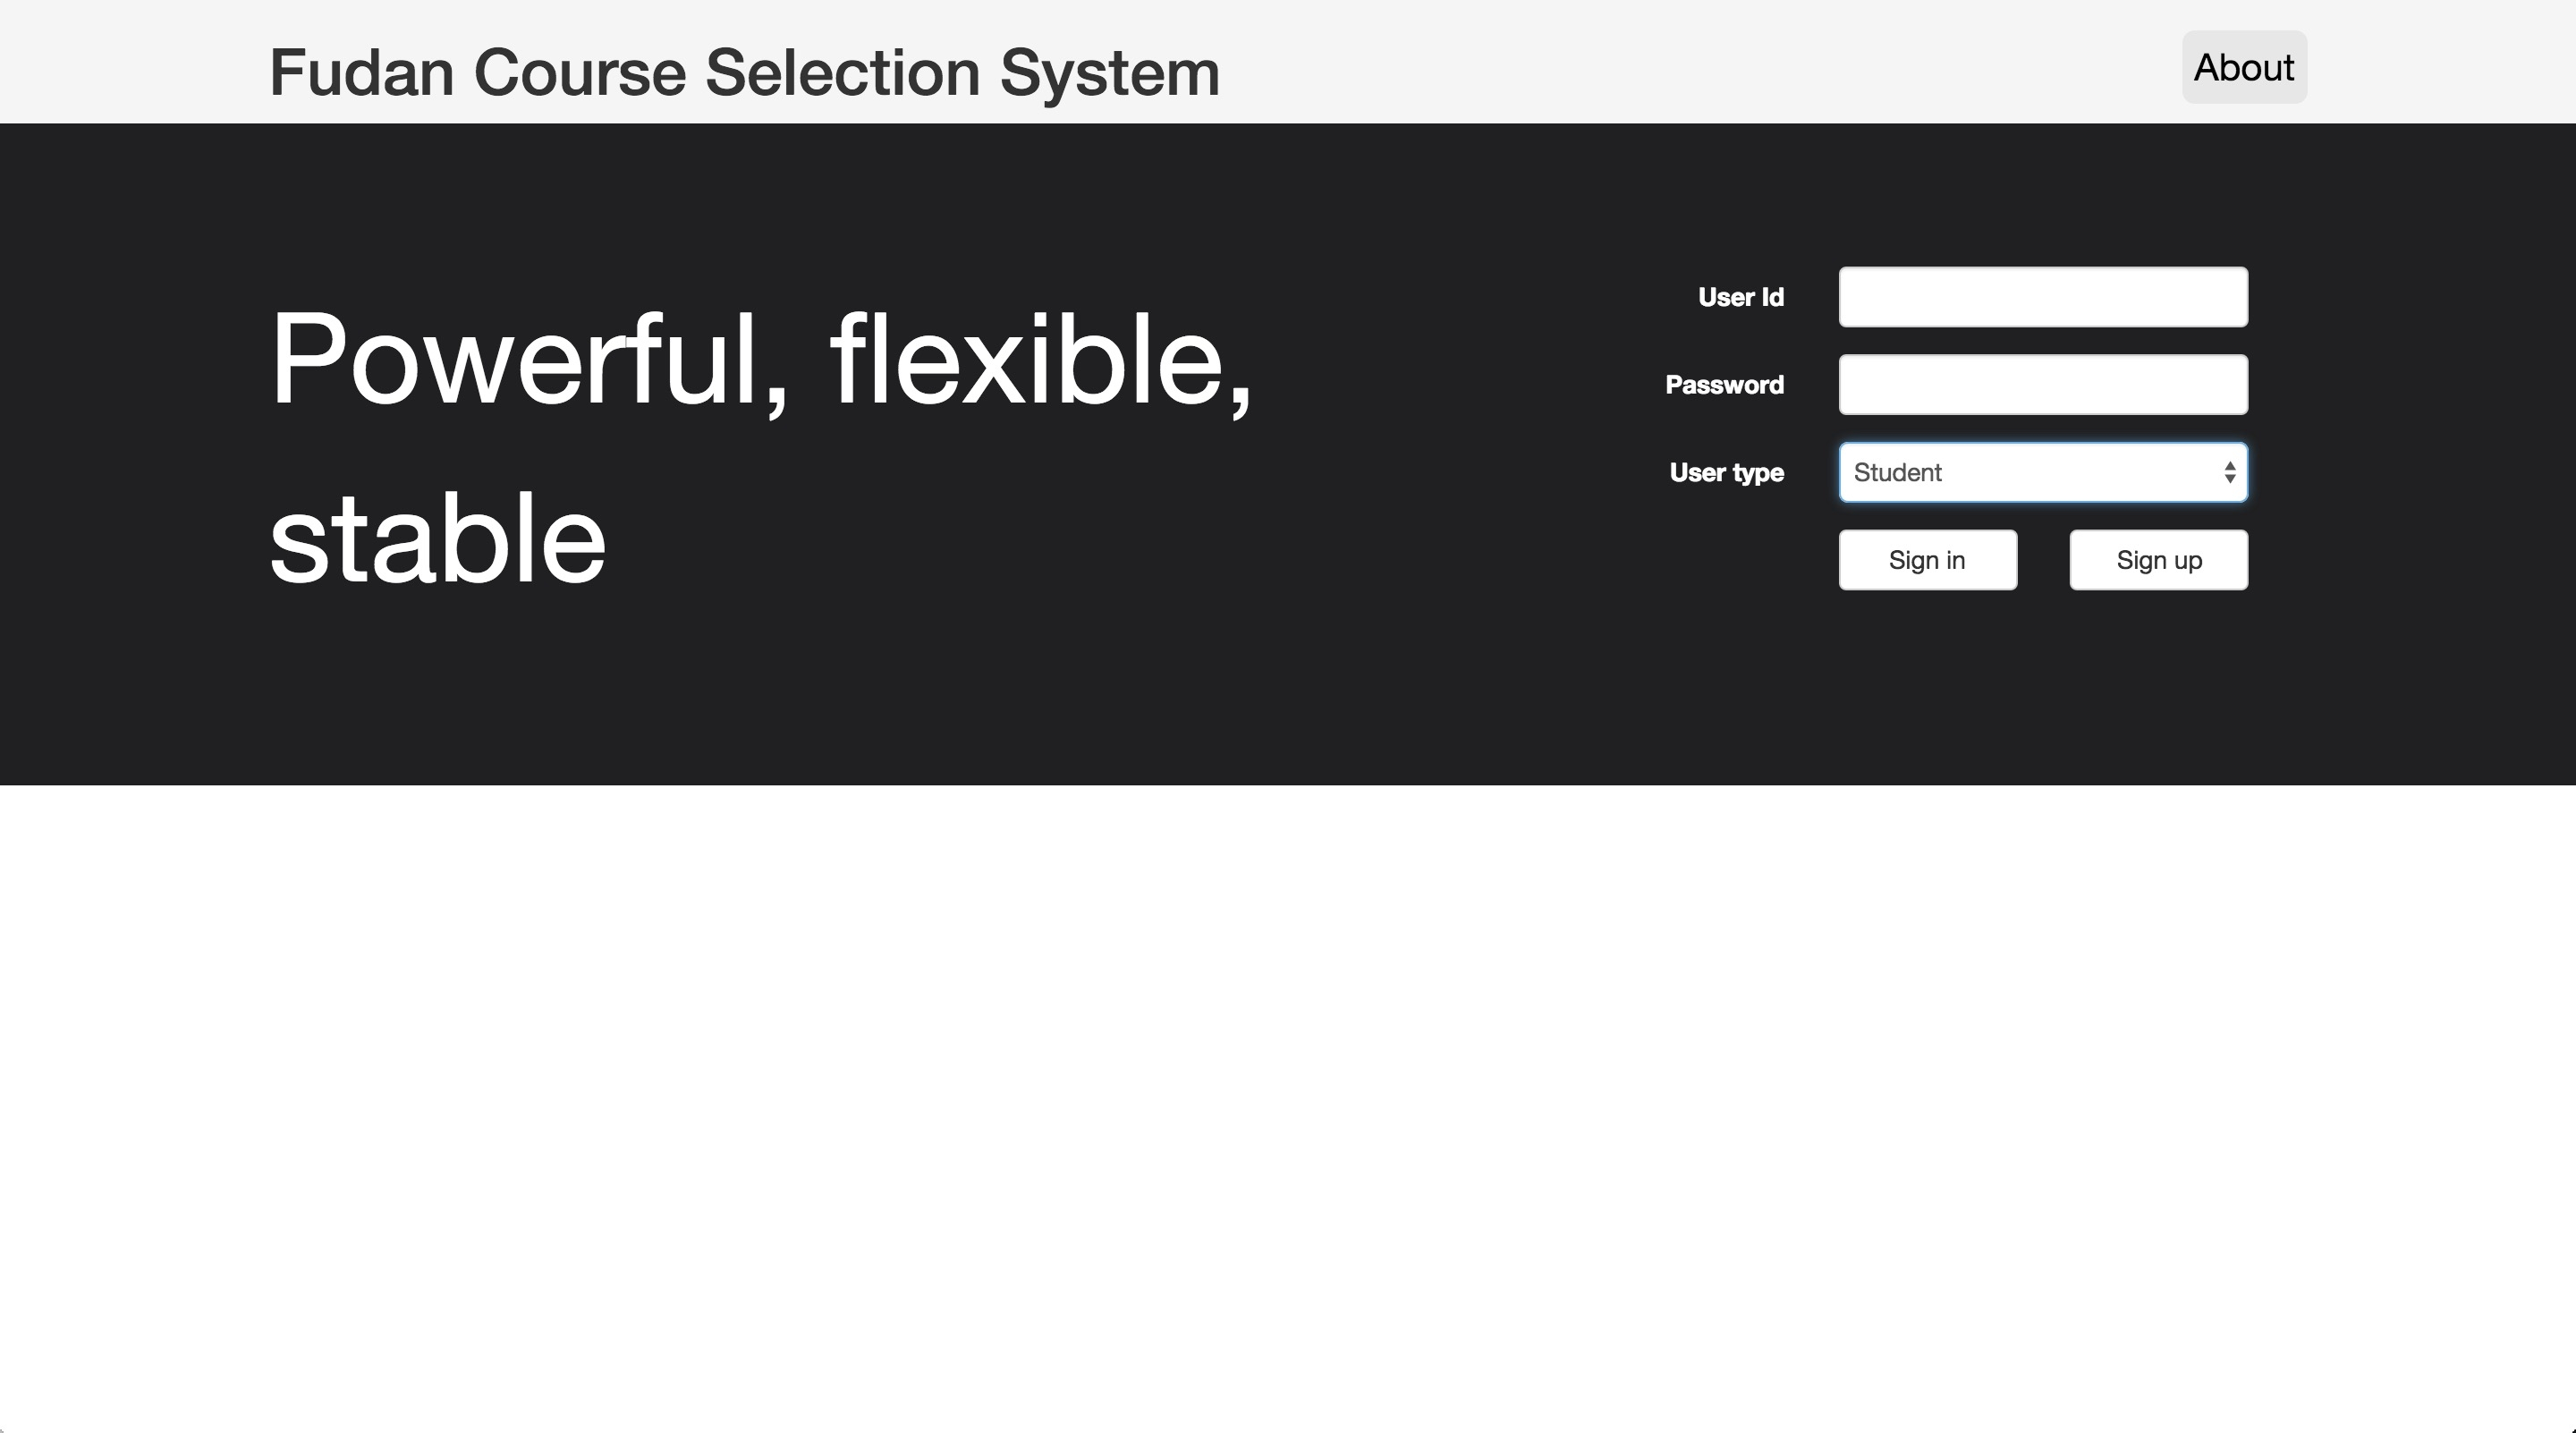
\includegraphics[width=6in]{overview}
		\caption{Index}
	\end{figure}

	图1即为选课系统的首页,学生、教师、教务员均可通过账号和密码进行登录。登录后,可以点击右上角的账号进行登出和修改个人信息,修改界面如图4所示。同时,系统允许用户进行注册。

	\begin{figure}[ht]
		\begin{minipage}{0.5\textwidth}
			\centering
			
\includegraphics[width=2.2in]{usertype}
			\caption{User Type}
		\end{minipage}%
		\begin{minipage}{0.5\textwidth}
			\centering
			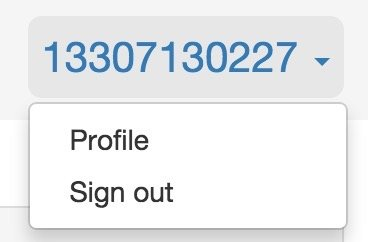
\includegraphics[width=2.2in]{user}
			\caption{User}
		\end{minipage}
	\end{figure}

	\begin{figure}[ht]
		\centering
		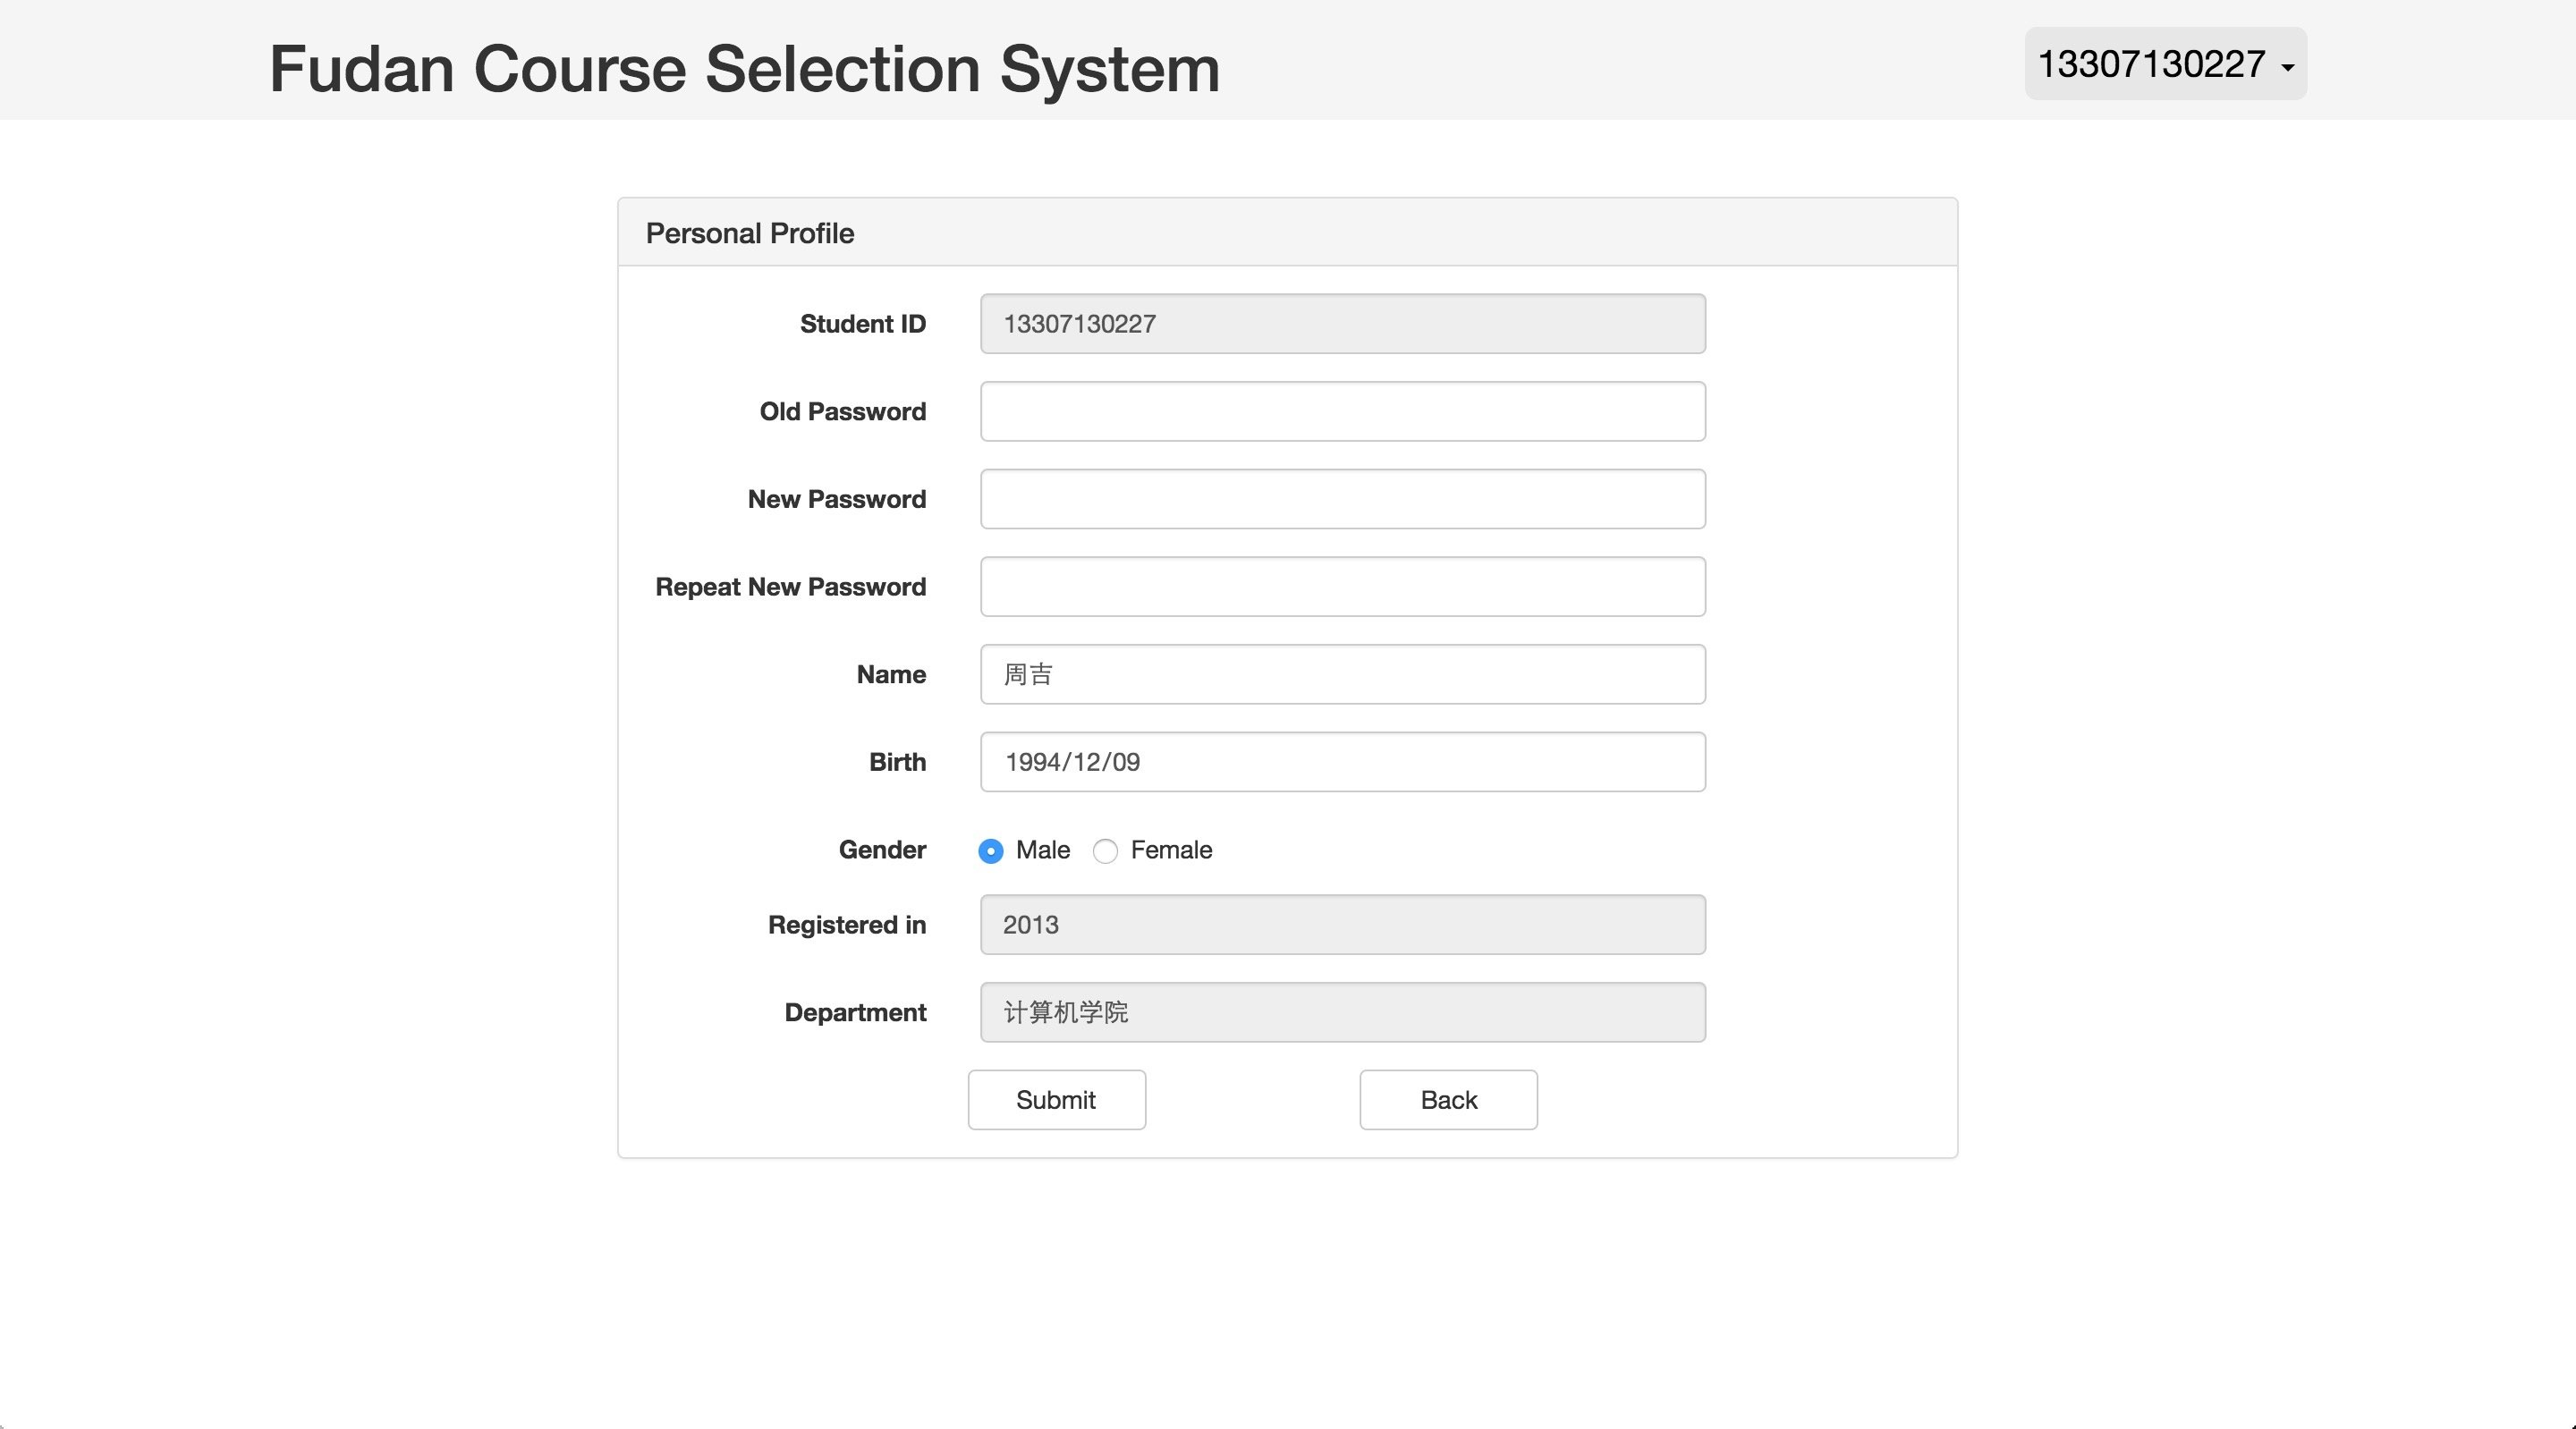
\includegraphics[width=6in]{stupro}
		\caption{Profile}
	\end{figure}

\newpage
\subsubsection{学生}

	学生登录后的界面如图5所示,学生可以查询自己的课表及可选课程,也可以通过选课号进行选课、退课及课程信息查询。

	图6至图11展示了对于选课号的操作,系统将会判断选课号是否存在,以及学生是否选择该课程。对于选课,系统还会自动判断课程之间是否有时间冲突。

	图12是对上课时间和上课地点的查询,在课程查询中,把鼠标移到课程号上的时候,会显示该课程的上课时间和上课地点。

	
	\begin{figure}[ht]

		\centering
		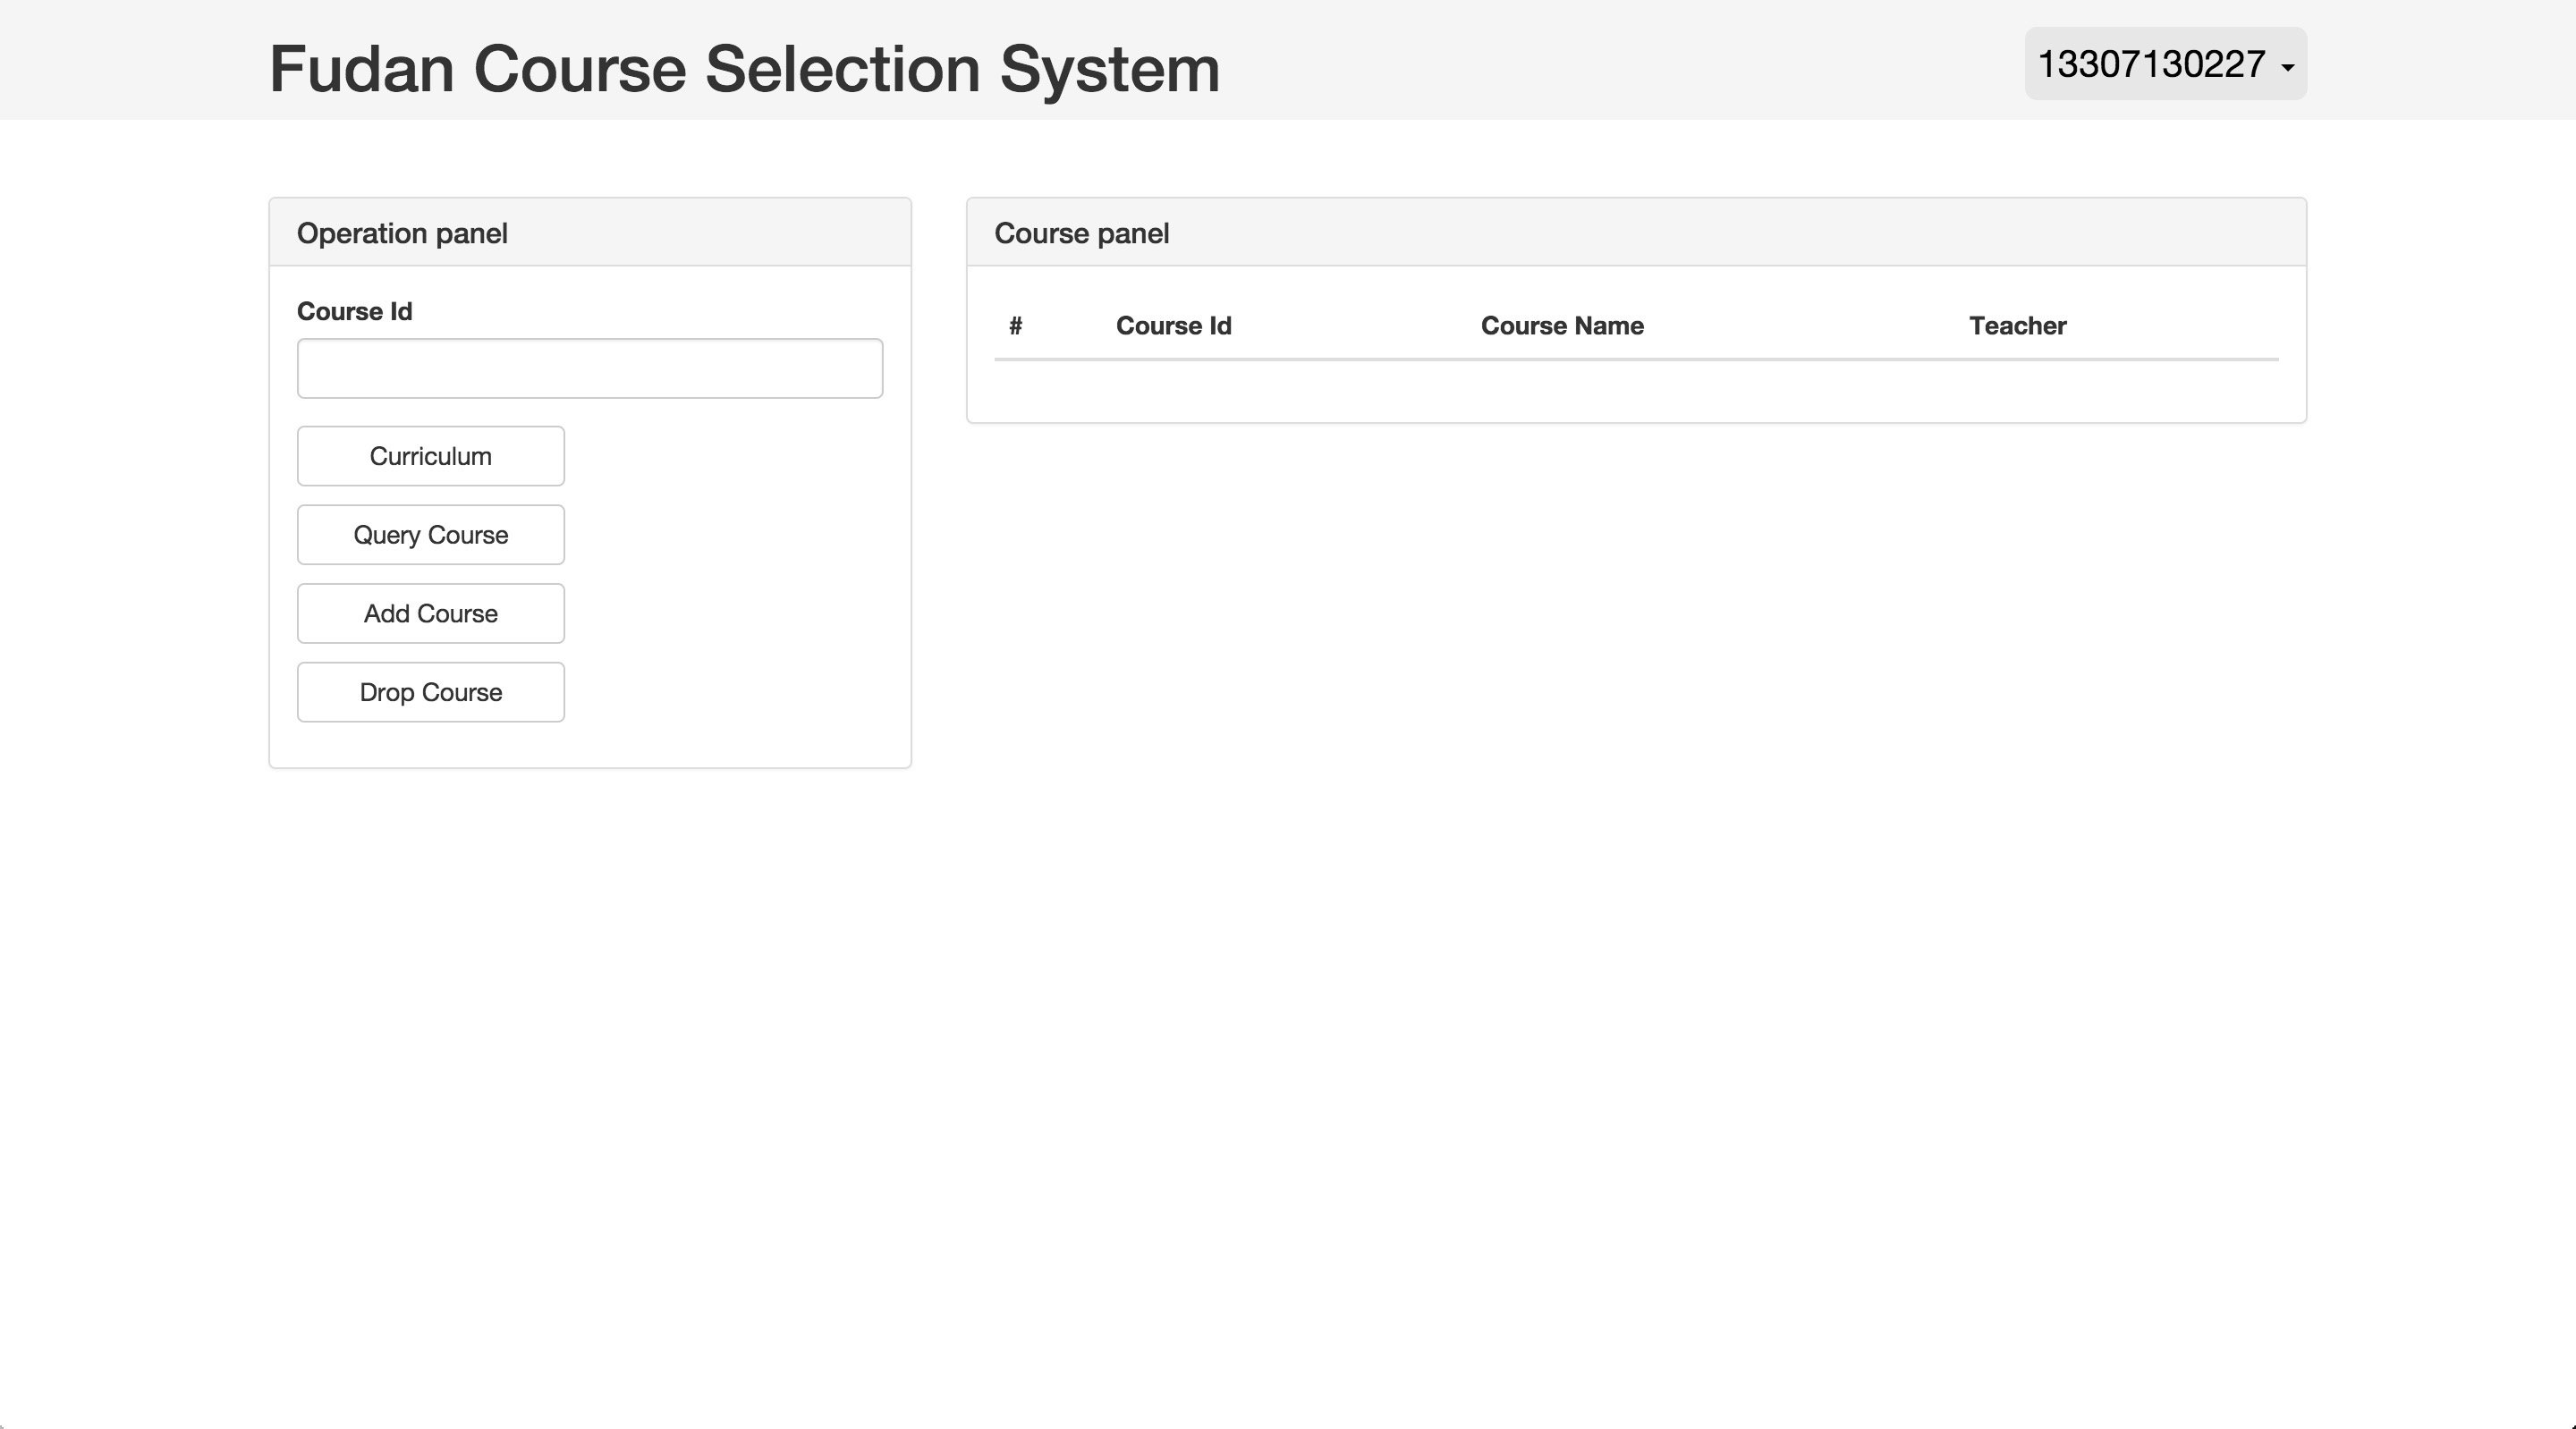
\includegraphics[width=6in]{student}
		\caption{student}

		\vspace{0.8cm}

		\begin{minipage}{0.5\textwidth}
			\centering
			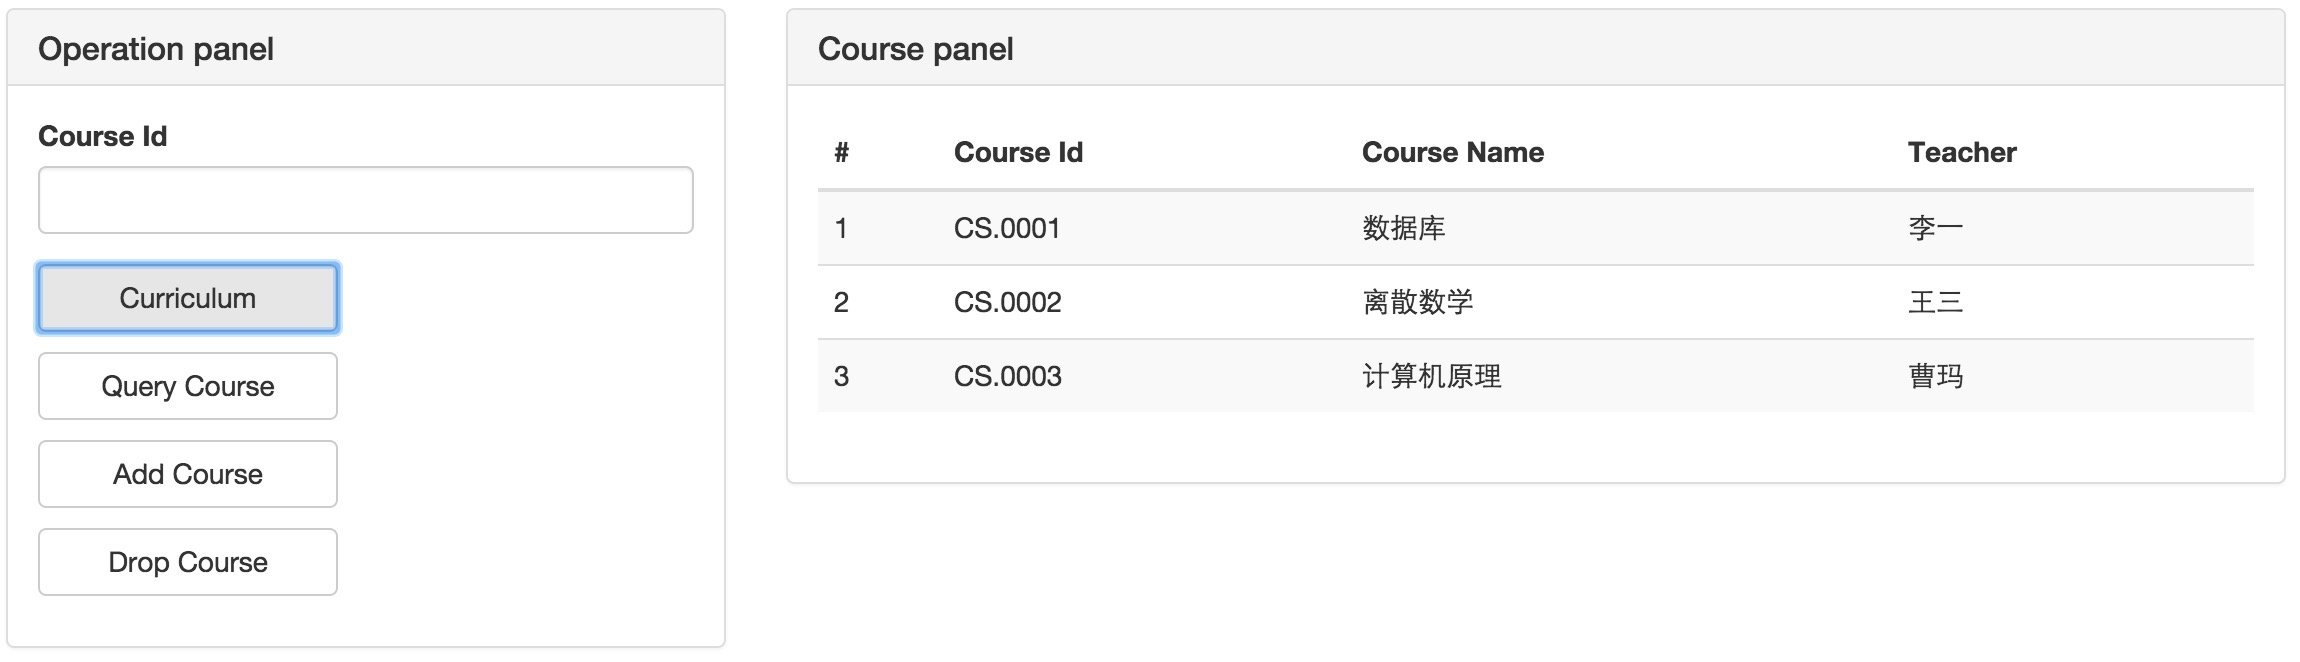
\includegraphics[width=3in]{curriculum}
			\caption{Curriculum}
		\end{minipage}%
		\begin{minipage}{0.5\textwidth}
			\centering
			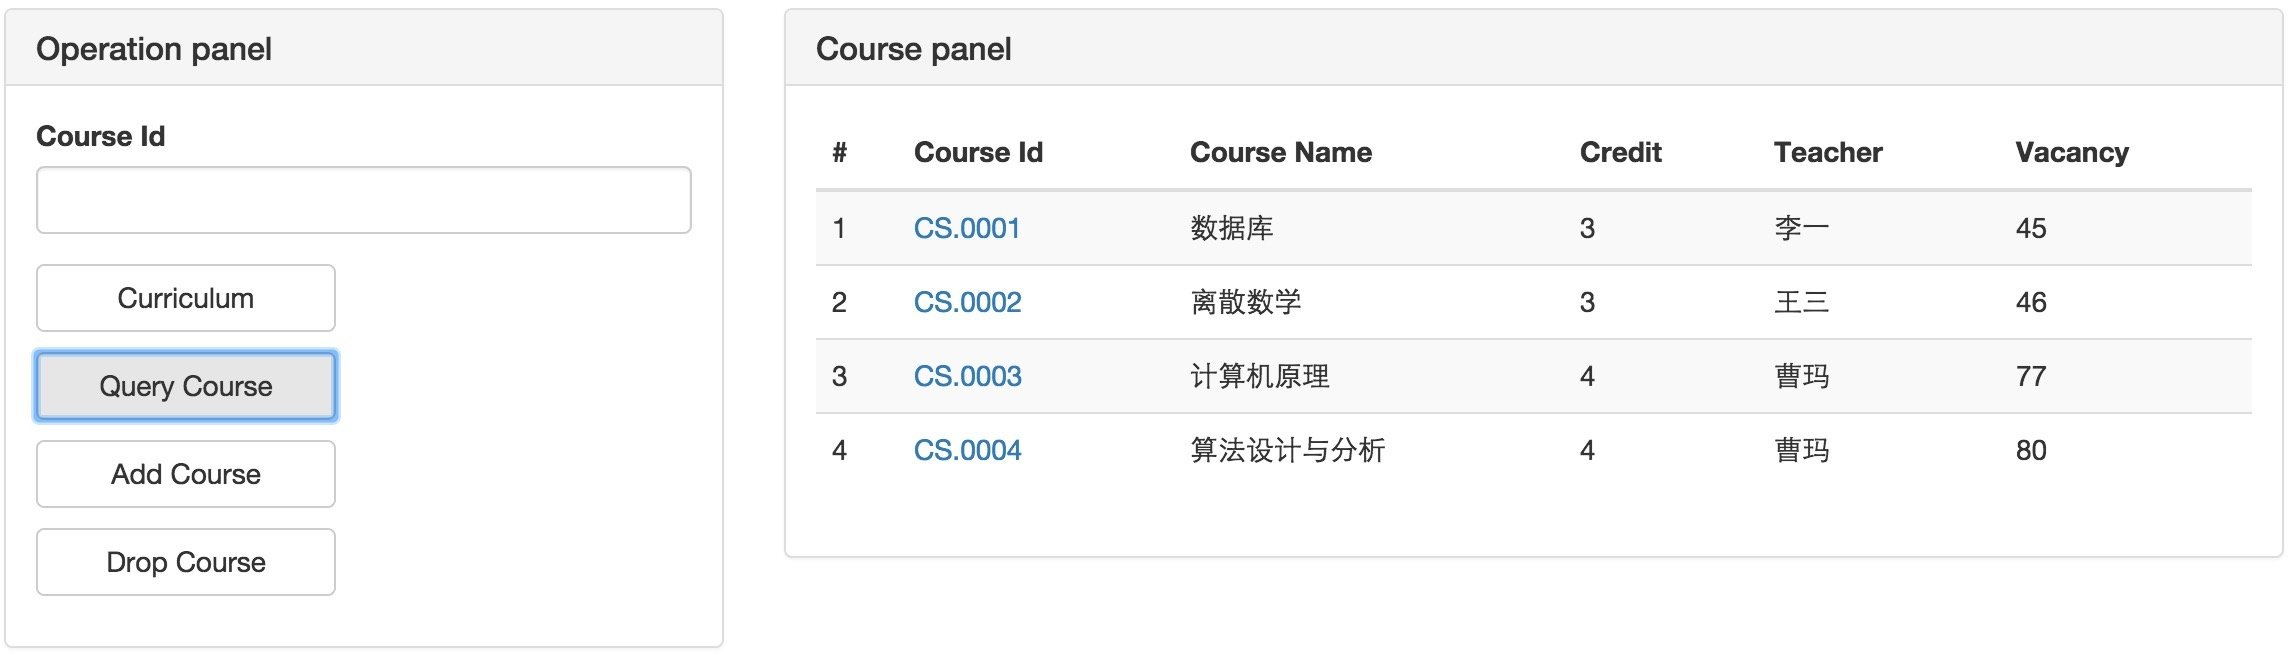
\includegraphics[width=3in]{query}
			\caption{Query}
		\end{minipage}
	\end{figure}
	\vspace{0.8cm}

	\begin{figure}[ht]

		\begin{minipage}{0.3\textwidth}
			\centering
			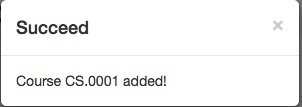
\includegraphics[width=1.5in]{add}
			\caption{Add Course}
		\end{minipage}%
		\begin{minipage}{0.4\textwidth}
			\centering
			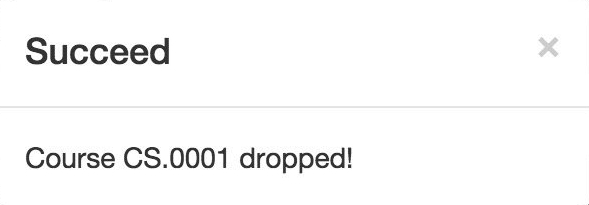
\includegraphics[width=1.5in]{drop}
			\caption{Drop Course}
		\end{minipage}%
		\begin{minipage}{0.3\textwidth}
			\centering
			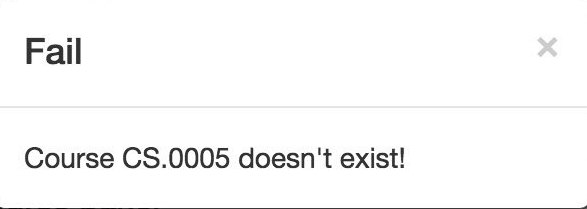
\includegraphics[width=1.5in]{notexist}
			\caption{Course Not Exist}
		\end{minipage}
	\end{figure}
	\vspace{0.8cm}

	\begin{figure}

		\begin{minipage}{0.4\textwidth}
			\centering
			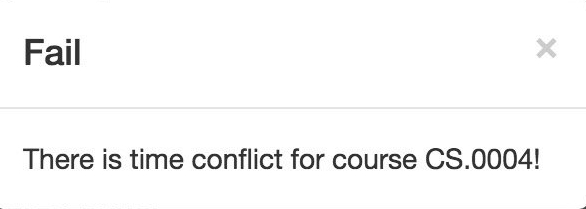
\includegraphics[width=2in]{timeconflict}
			\caption{Course Time Conflict}
		\end{minipage}%
		\begin{minipage}{0.6\textwidth}
			\centering
			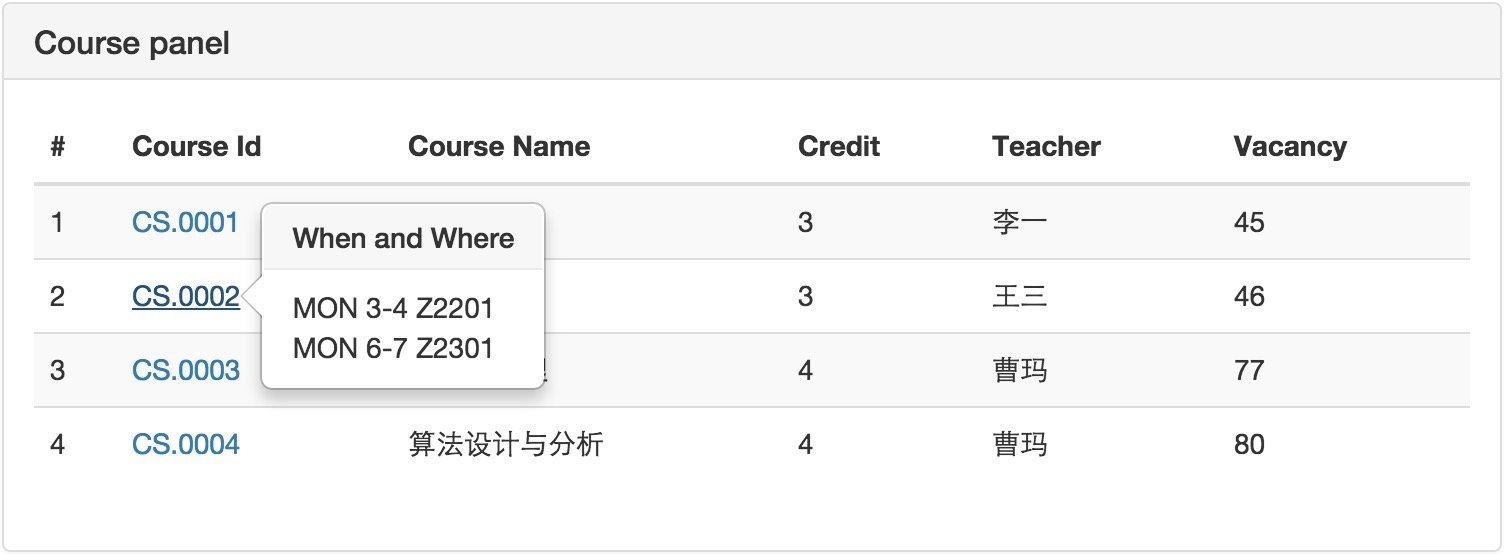
\includegraphics[width=2in]{showtime}
			\caption{Query When Where}
		\end{minipage}

		\vspace{0.8cm}
	\end{figure}

\newpage
\subsubsection{教师}

	\begin{figure}[h]
		\begin{minipage}{0.5\textwidth}
			\centering
			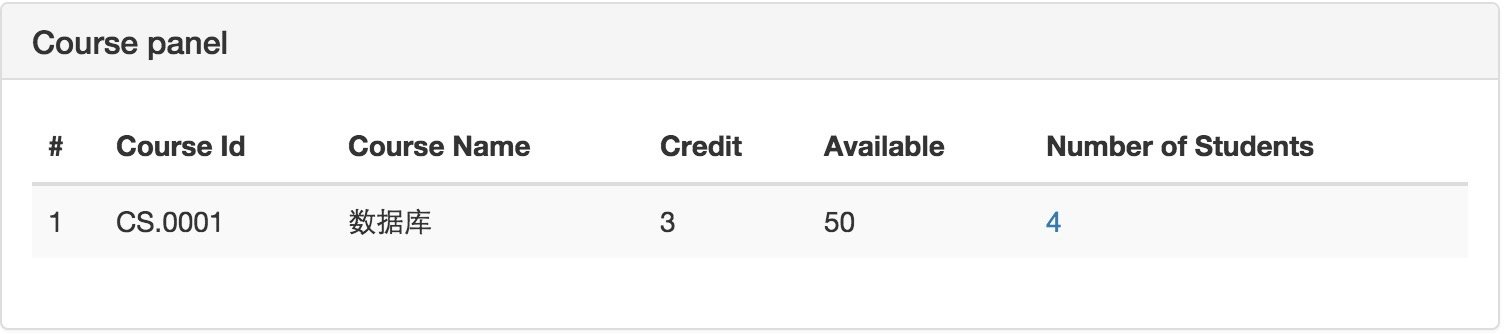
\includegraphics[width=2.5in]{teacher}
			\caption{Teacher}
		\end{minipage}%
		\begin{minipage}{0.5\textwidth}
			\centering
			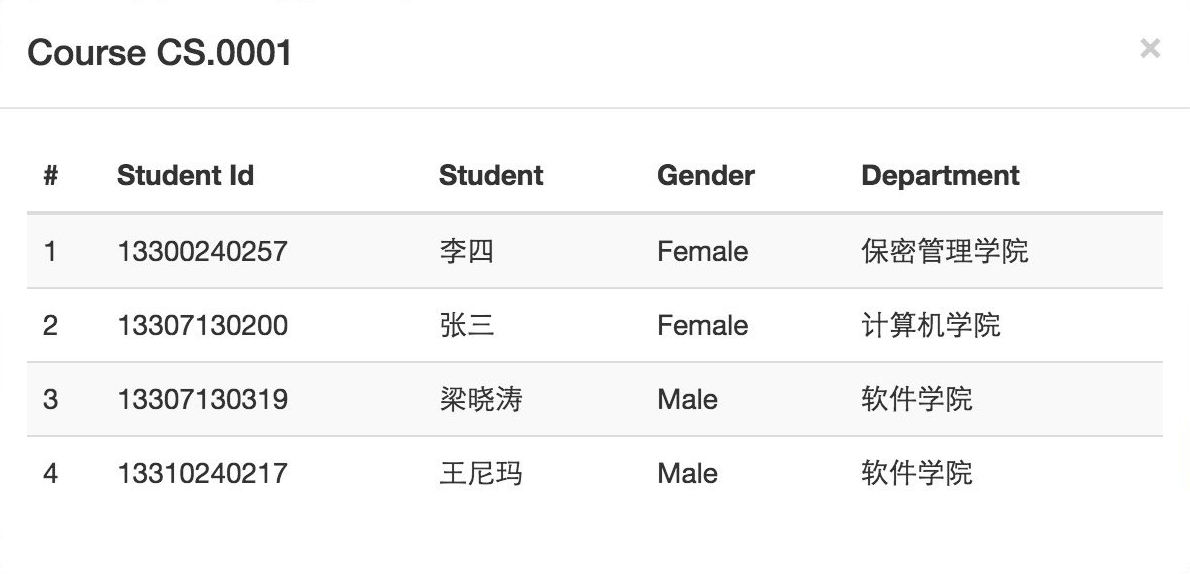
\includegraphics[width=2.5in]{adteacou}
			\caption{Student List}
		\end{minipage}
			\vspace{0.8cm}

	\end{figure}

	教师页面的基本功能为查看该教师所授课程列表,如图13、图14所示。同时,教师还可以查询他的课程的选课名单,点击图中的人数,即可显示该课程的选课名单。

\newpage
\subsubsection{教务员}

	\begin{figure}[h]
		\centering
		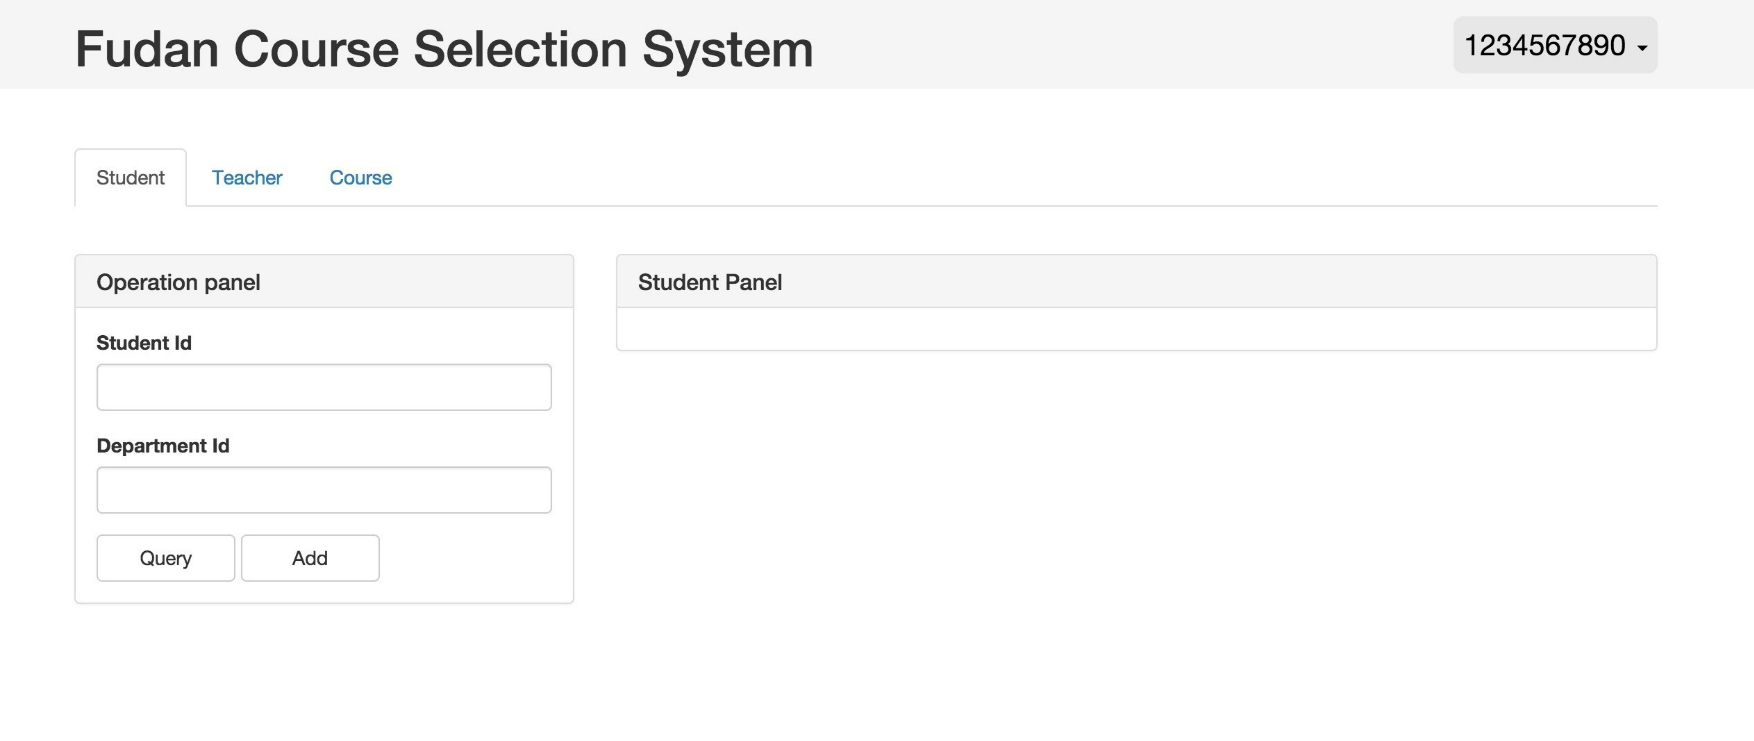
\includegraphics[width=6in]{adover}
		\caption{Admin}
	\end{figure}

	教务员拥有对学生、教师和课程的添加、删除及修改权限。图16至图20显示,教务员可以添加或删除学生、教师及课程,也可以单独修改学生、教师和课程的信息,同时,教务员也可以为学生选课。

	\begin{figure}[h]
		\begin{minipage}{0.5\textwidth}
			\centering
			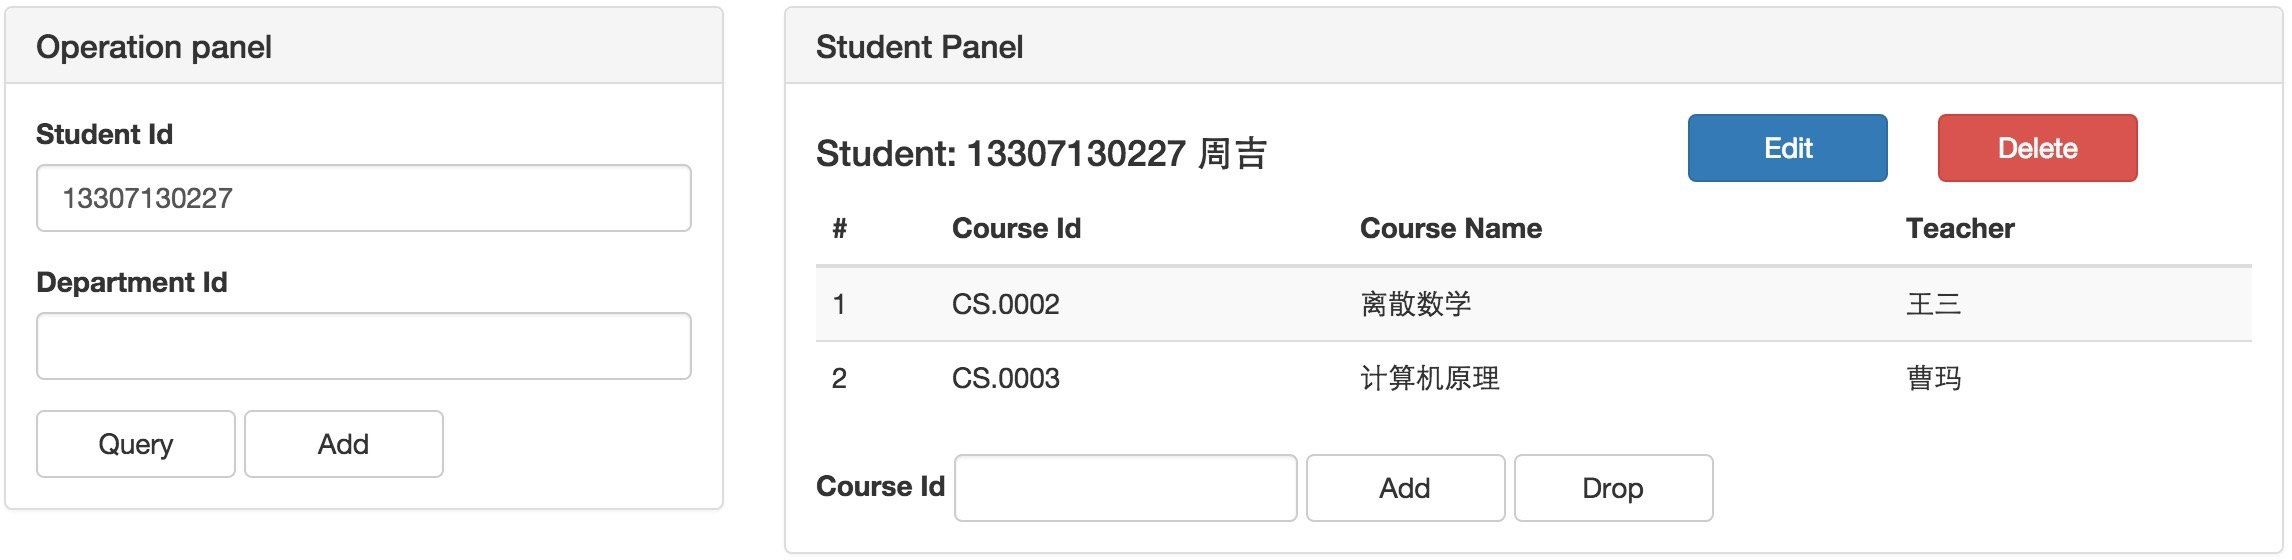
\includegraphics[width=3in]{adstu}
			\caption{Admin Student}
		\end{minipage}%
		\begin{minipage}{0.5\textwidth}
			\centering
			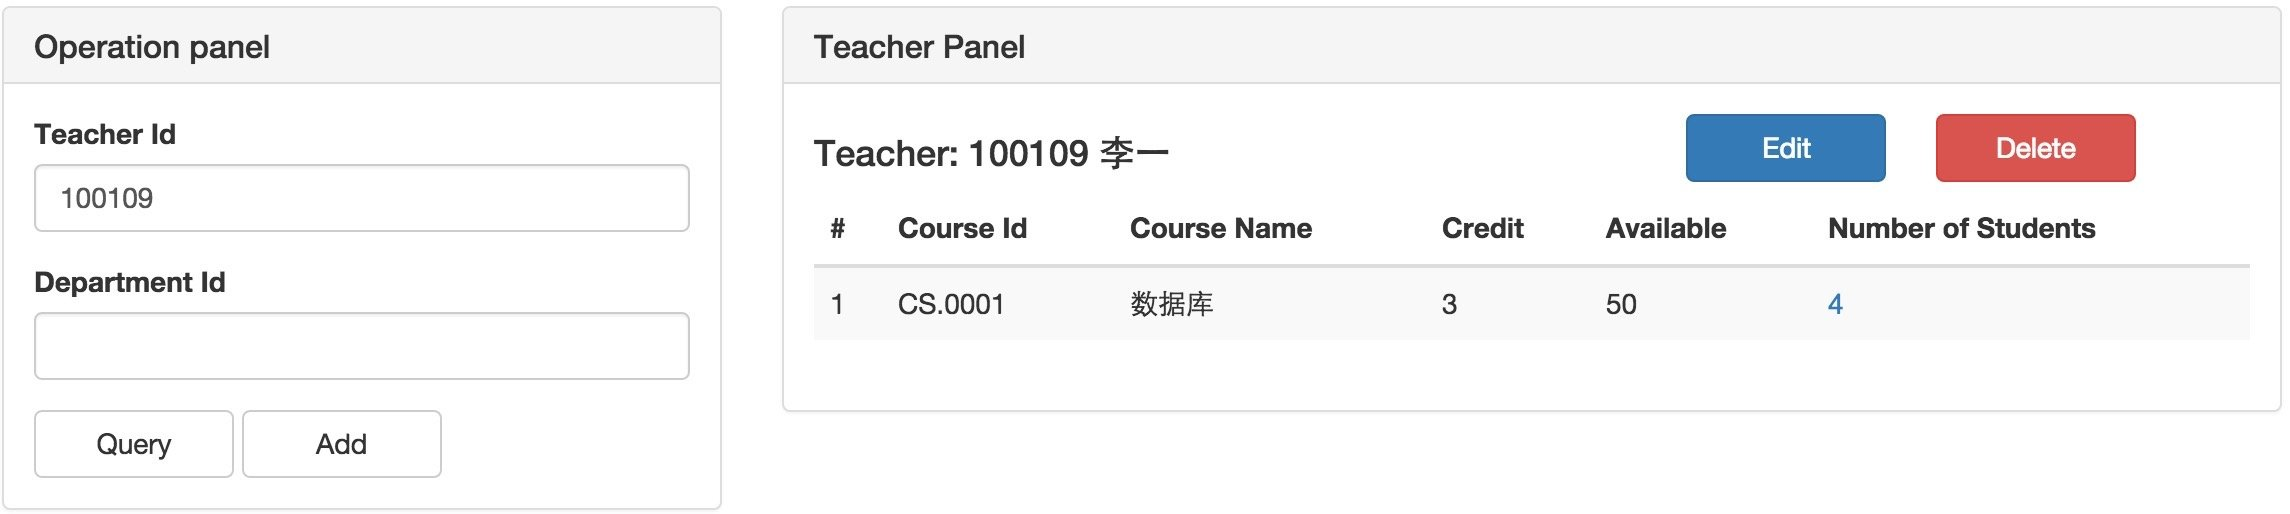
\includegraphics[width=3in]{adtea}
			\caption{Admin Teacher}
		\end{minipage}

			\vspace{0.8cm}

		\begin{minipage}{0.5\textwidth}
			\centering
			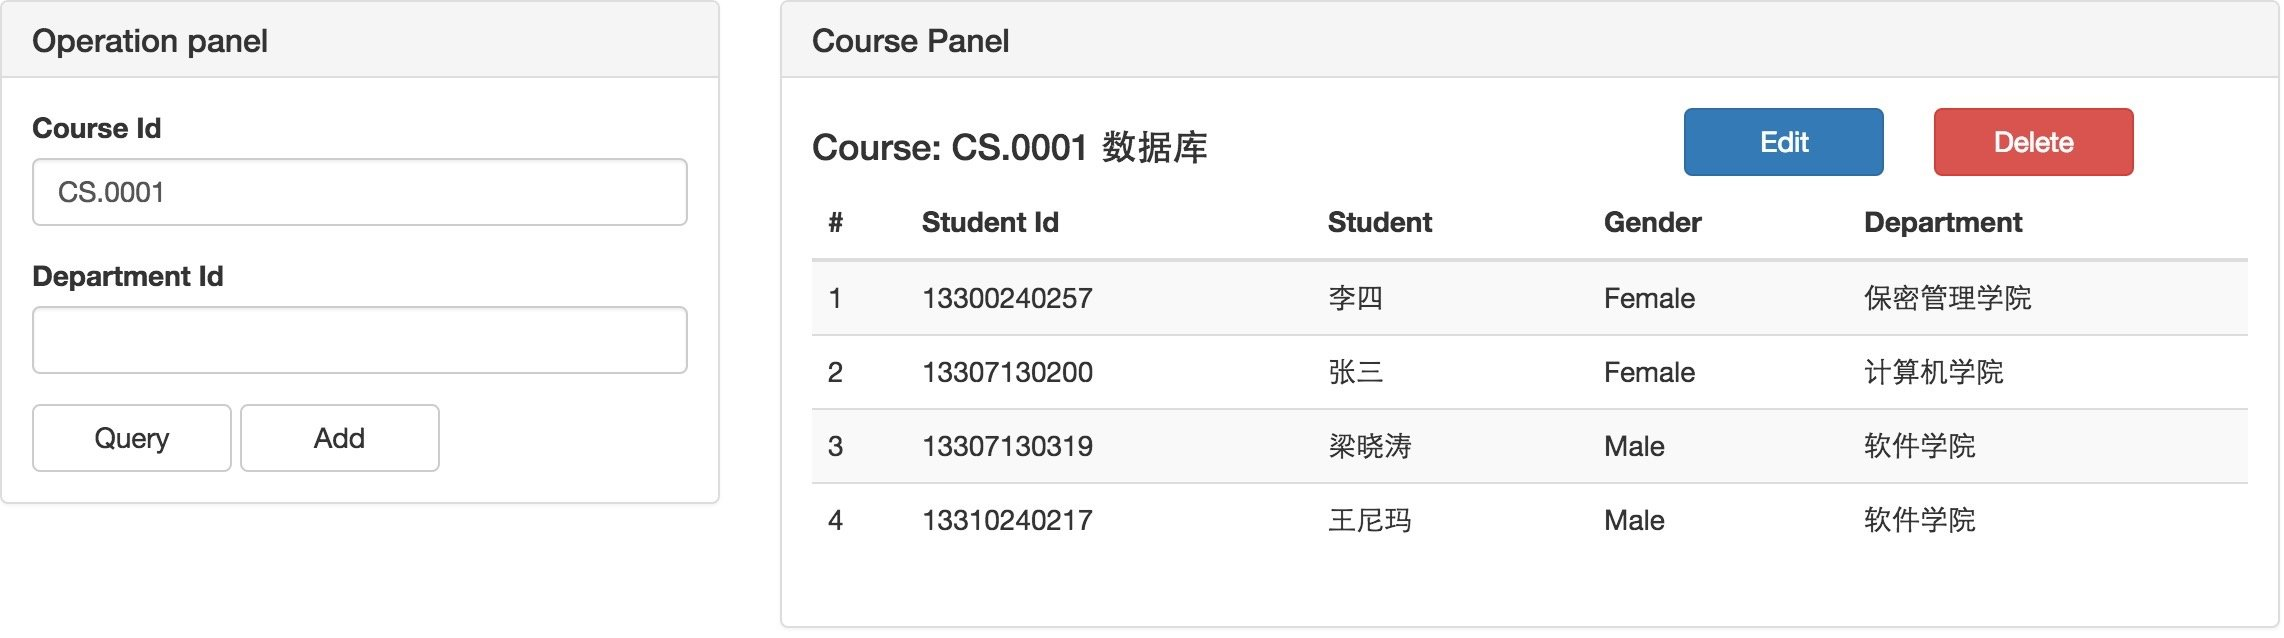
\includegraphics[width=3in]{adcou}
			\caption{Admin Course}
		\end{minipage}%
		\begin{minipage}{0.5\textwidth}
			\centering
			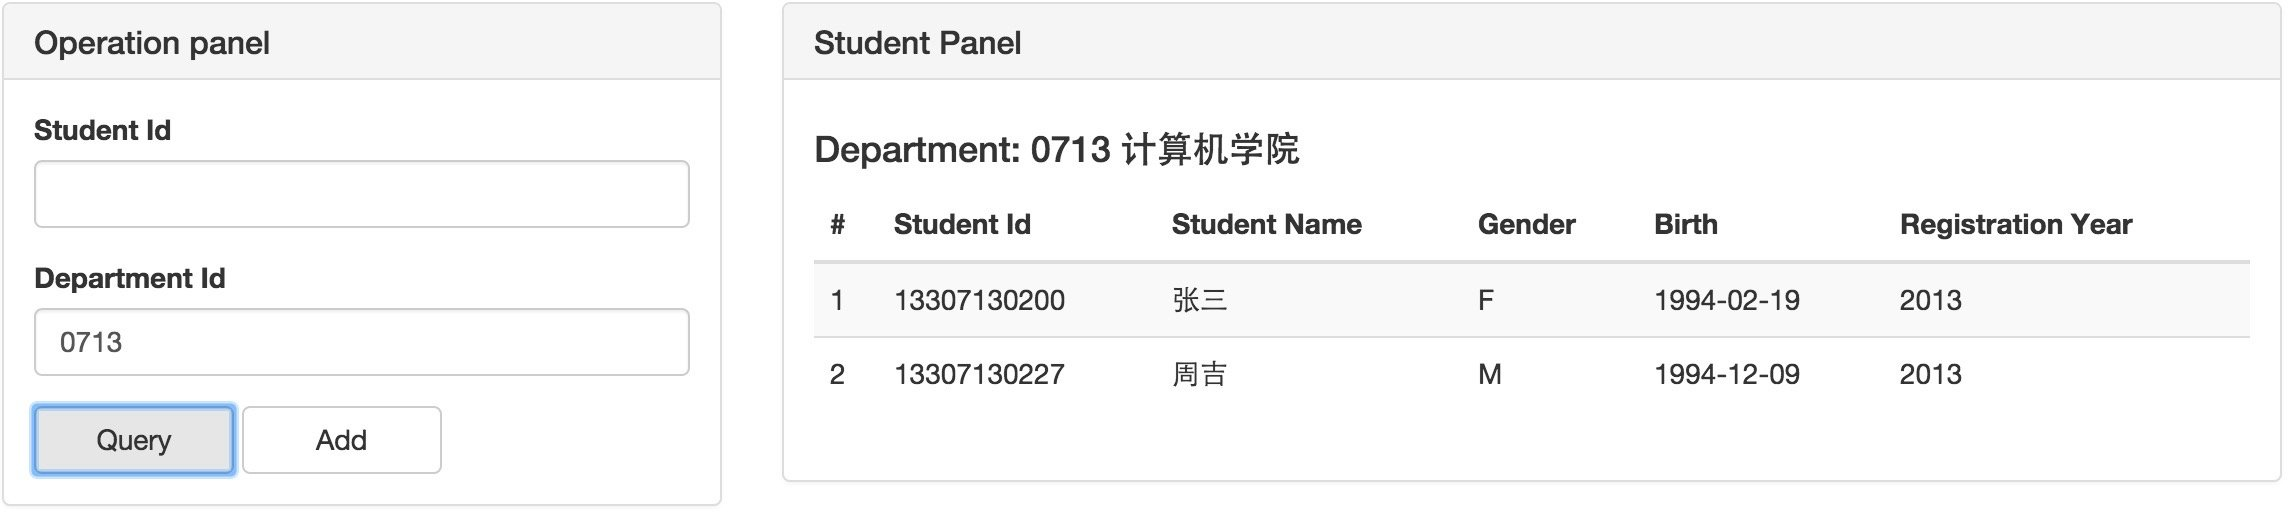
\includegraphics[width=3in]{addep}
			\caption{Group By Department}
		\end{minipage}

			\vspace{0.8cm}

		\centering
		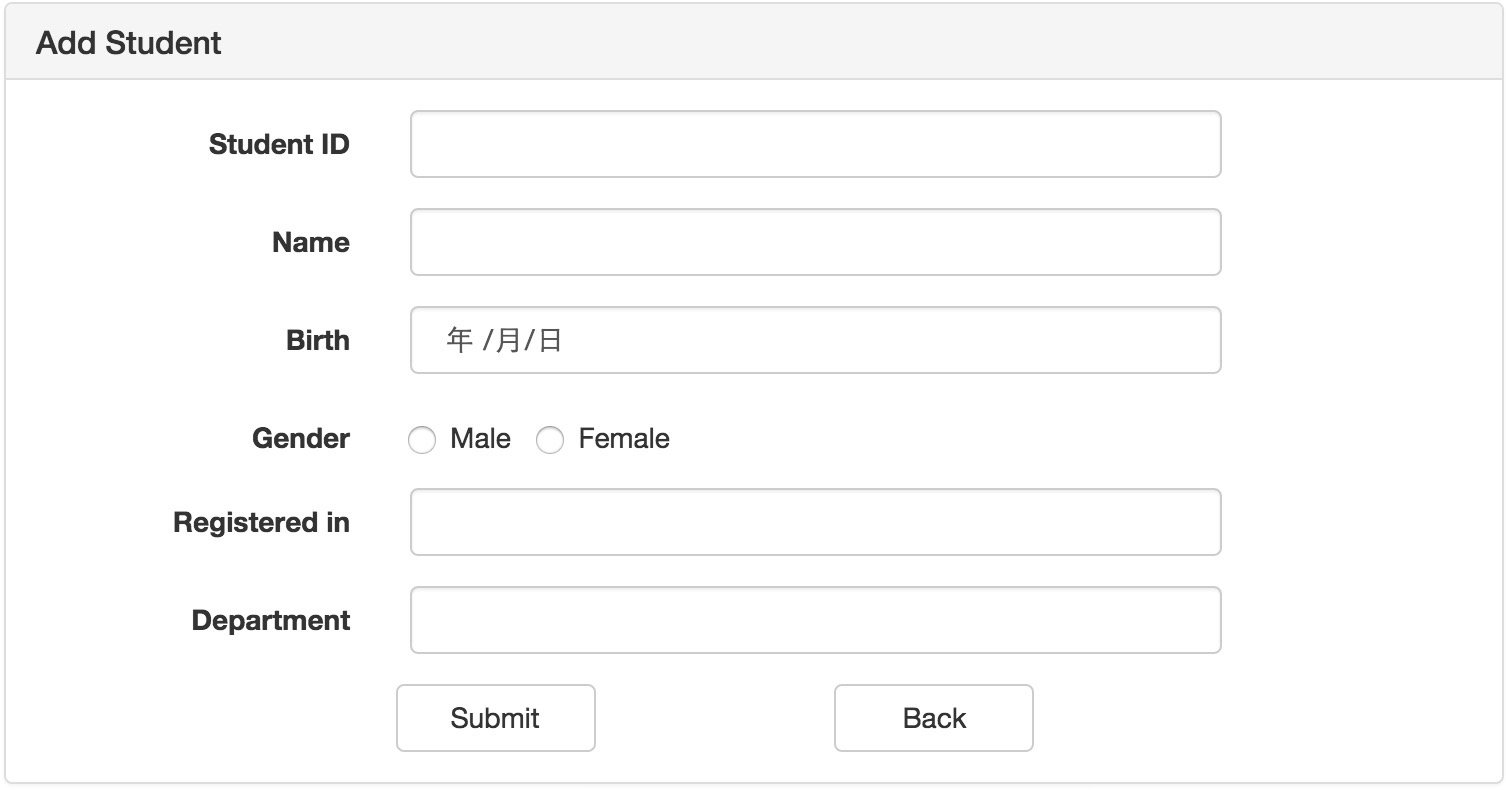
\includegraphics[width=4in]{adadd}
		\caption{Add Person}
	\end{figure}

\newpage
\section{数据库的概念设计}

\subsection{设计思路}
我们分析了选课系统的要求,首先初步确定了问题的所需的实体:学生、教师、课程、院系、教务员。显然,院系和学生之间有一对多的联系,院系与教师之间有一对多的联系,教师和课程之间也有一对多的联系。而学生与课程之间则是一个多对多的联系,从而需要将其转换为一个实体。进一步分析这个模式,发现每个课程有多个上课时间和多个上课地点,于是把上课时间和上课地方拆分为两个实体,它们与课程之间有一个三元的联系。至此,这个关系模式已经设计完成,我们可以据此画出ER图。

\subsection{ER图}
	\includegraphics[width=6in]{ER图}

\section{数据库的逻辑设计}

\subsection{表关系}
由上述ER图可知,一共有7个实体,其结构如下:
\begin{itemize}
    \item 学生(\underline{学号},登陆密码,姓名,出生年月,性别,入学年份)
    \item 教师(\underline{工号},登陆密码,姓名,出生年月,性别,职称)
    \item 课程(\underline{选课号},课程名,人数,学分)
    \item 学院(\underline{编号},学院名,院长)
    \item 教务员(\underline{编号},密码,姓名,出生年月,性别)
    \item 上课时间(\underline{时间})
    \item 上课地点(\underline{地点})
\end{itemize}

实体之间有5个联系,其中有3个1:N的联系,1个M:N的联系,1个1:N:N的联系,联系的属性如下:
\begin{itemize}
    \item 学生所属院系(院系编号,学号)
    \item 教师所属院系(院系编号,工号)
    \item 课程教师信息(选课号,工号)
    \item 选课信息(选课号,学号,成绩)
    \item 课程安排(选课号,上课时间,上课地点)
\end{itemize}

根据转换规则,我们可以将M:N的联系和1:M:N的联系转换为实体,因此,上述ER图可以转换为如下关系模式:
\begin{itemize}
    \item 学生(\underline{学号},登陆密码,姓名,出生年月,性别,入学年份,\uwave{院系编号})
    \item 教师(\underline{工号},登陆密码,姓名,出生年月,性别,职称,\uwave{院系编号})
    \item 课程(\underline{选课号},课程名,人数,学分,\uwave{教师工号})
    \item 学院(\underline{编号},学院名,院长)
    \item 教务员(\underline{编号},密码,姓名,出生年月,性别)
    \item 选课信息(\underline{\uwave{选课号},\uwave{学号}},成绩)
    \item 课程安排(\underline{\uwave{选课号},\uwave{上课时间}},上课地点)
\end{itemize}

\subsection{建表语句}

\lstinputlisting{../SQL/CreateTable.sql}

\section{实验总结}

本实验是第一次由自己完成从设计数据库开始到完成一个成熟系统的一系列过程。加深理解了数据库的设计、ER图及ER图到关系模式的转换。通过实验,熟练掌握了Mysql以及SQL语句的使用,学会了对数据库的创建、修改、查询以及使用。同时,由于系统的需要,锻炼了嵌入式SQL的使用能力,也对PHP及HTML有了一定的掌握。在此次实验中,也暴露出对数据库这门学科的一些问题,并在实验的调试及讨论中获得了解决。作为本学期第一次实验,为编写数据库相关程序提供了经验,也为第二次实验打下了基础。

\end{document}
